\chapter{Arquitetura}

Delineado os objetivos, vamos proceder para a elaboração da arquitetura do serviço, falando dos componentes num alto nível de abstração antes de mergulhar nos detalhes tecnológicos e de implementação. Aqui vamos detalhar com mais rigor as funcionalidades base do sistema assim como as entidades que o compõem.

\section{Sistema}

O \textit{middleware}, devido ao seu tamanho e à sua complexidade, não será composto apenas por um único elemento de software, sendo composto por vários elementos mais concisos, cada um resolvendo um conjunto de problemas. Neste caso iremos dividi-lo em duas partes, \textit{hub} e \textit{api}, dois componentes de software que fornecem APIs RESTful , uma para uso interno e outra para uso externo respetivamente, ambas seguindo as recomendações de Leonard Richardson no seu livro sobre serviços web \textit{RESTful} \cite{richardson2013restful}. Além destes dois elementos que compõem o \textit{middleware}, também serão desenvolvidas as simulações dos dispositivos, pequenas aplicações que irão simular o funcionamento dos diversos tipos de dispositivos, e por fim, uma aplicação cliente que faça uso de todas as funcionalidades oferecidas por esta plataforma.

\subsection{Hub}

O \textit{hub} consiste no conceito \textit{edge device} que já foi abordado anteriormente, um dispositivo que fornece um interface para interagir com os dispositivos do utilizador. Este componente deverá fornecer camadas de compatibilidade para diversos tipos de dispositivos, de modo a resolver o problema relativo à heterogeneidade dos dispositivos IoT.

Este componente será pré-instalado e configurado em dispositivos que deverão depois ser fornecidos aos utilizadores (num caso de utilização em massa). Neste caso de demonstração académica, será utilizado um Raspberry PI para simular este dispositivo. O serviço irá correr como um \textit{daemon} nestes dispositivos, sendo iniciado durante o processo de \textit{boot}.

Este componente deverá fornecer uma API HTTP RESTtful, que permita interagir com os dispositivos no espaço casa, de acesso exclusivo à \textit{api}. O \textit{hub} deverá ter métodos \textit{GET} e \textit{PUT}, para manipular os dispositivos. Este métodos deverão ser acompanhados de parâmetros que identificam um dispositivo, como por exemplo, endereço IP, porta de acesso, e outros parâmetros exclusivos a um dispositivo. Estes parâmetros deverão ser obtidos em parte pelo sistema de descoberta de dispositivos presente neste componente, que procura no espaço casa dispositivos compatíveis, retornando os seus parâmetros de acesso.

O \textit{hub} é portanto \textit{stateless}, ou seja, não armazena nenhum tipo de informação ao longo do seu funcionamento, essa função está ao encargo da \textit{api}, que vamos detalhar já de seguida. Além disso, este componente irá ser exposto através de um software de \textit{tunneling}, que como já foi visto anteriormente, é uma melhor opção do que UPNP e \textit{port-forwarding} para a exposição de recursos em redes locais.

\subsection{Api}

A \textit{api} contém toda a lógica relacionada com utilizadores, casas, dispositivos e a manipulação de cenários e tarefas. Este componente é o típico servidor aplicacional com acesso a base de dados que contém toda a lógica de negócio do sistema. A \textit{api}, tal como o \textit{hub}, deverá fornecer uma API HTTP, seguindo também uma arquitetura \textit{REST}. Esta API será de acesso público, contrastando com a API do \textit{hub} que é de acesso exclusivo ao \textit{middleware}.

Dado que o \textit{hub} é um componente \textit{stateless}, a \textit{api} deverá armazenar os parâmetros de acesso aos dispositivos. Além disso, todos as funcionalidades do \textit{hub} devem ser acessíveis a partir da API, efetuando reencaminhamento das aplicações clientes para o \textit{hub}.

Tudo isto irá consistir num sistema de tamanho médio composto essencialmente de operações \textit{CRUD}, tornando-se mais complexo na área das tarefas automatizadas, onde provavelmente se deverá investir em alguma \textit{framework} de \textit{background jobs} para monitorizar e controlar dispositivos assincronamente, sem criar carga adicional no servidor aplicacional.

Obviamente, os recursos irão pertencer a uma entidade ''utilizador'', sendo necessário algum tipo de autenticação para aceder aos mesmos, que em princípio será \textit{token-based}.
\subsection{Simuladores de Dispositivos}

Estes simuladores têm como função emular o funcionamento de dispositivos do mundo real. Isto permite proceder a uma demonstração completa sem ter que adquirir vários tipos de dispositivos diferentes. Neste preciso caso os dispositivos deverão fornecer APIs HTTP Restful, um standard bastante utilizado na indústria. Para demonstrar a compatibilidade de vários protocolos, também serão desenvolvidos alguns exemplos em CoAP.

\subsection{\textit{Wrapper} da API}

É boa prática que após o desenho e conceção de uma API à base de HTTP e JSON se desenvolvam \textit{wrappers} para as linguagens de programação mais comuns. Um wrapper essencialmente converte as chamadas à API utilizando HTTP para métodos ou funções da linguagem respetiva.

Por exemplo, temos um recurso \textit{foo} disponível numa API HTTP \textit{Restful}, para efetuar a sua obtenção deveria ser feito algo como:

\begin{verbatim}
        HTTP GET -> /foo/1
\end{verbatim}

Um \textit{wrapper} converteria estas comunicações HTTP para métodos de uma linguagem de programação. Um \textit{wrapper} em Java provavelmente atuaria da seguinte maneira:

\begin{minted}{java}
        FooApiWrapper api = new FooApiWrapper(remoteHost);

        Foo foo = api.getFoo(1);
\end{minted}


Internamente o \textit{wrapper} faria a chamada à API remota e devolveria o resultado respetivo, um objeto em vez de uma resposta HTTP, fazendo toda a serialização automaticamente. Isto permite retirar uma grande porção de código que se iria repetir em todas as aplicações clientes. Neste caso, irá ser desenvolvido um \textit{wrapper} para a \textit{api} do \textit{middleware} na linguagem que for utilizada na aplicação cliente.

\subsection{Aplicação Cliente}

Como prova de conceito irá ser desenvolvida uma aplicação \textit{mobile}, em linguagem e sistema operativo mais à frente. A aplicação deverá fazer uma demonstração de todas as funcionalidades e operações que o \textit{middleware} implementa. Estas funcionalidades estão detalhadas na \hyperref[sec:funcionalidades]{secção} 2 do capítulo 4. Todos esses pontos serão aplicados ao resultado final da aplicação.

De notar que esta aplicação apenas foi desenvolvida para efeitos de demonstração, portanto, grande parte desta dissertação será, como é óbvio, sobre o \textit{middleware} e os seus componentes. Foi efetuado um esforço significativo para implementar boas práticas arquiteturais e de programação em todo o software desenvolvido, mas a aplicação cliente poderá ficar um pouco aquém dos restantes elementos.

\subsection{Visão Geral}

Um espaço casa deverá possui um \textit{hub} instalado, e a \textit{api} comunica com os dispositivos do espaço através deste equipamento. Com isto separamos uma componente complexa da \textit{api}, a camada de compatibilidade entre os diversos modelos de dispositivos, tornando todo o sistema mais manutenível.

\begin{figure}[H]
  \centering
        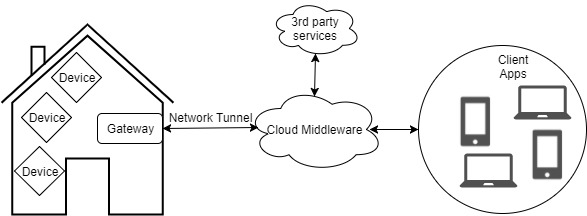
\includegraphics[scale=0.7]{img/arquitetura.jpg}
  \caption{Visão Geral dos Sistemas}
\end{figure}

Aqui o acesso aos dispositivos será abstraído graças ao \textit{software} que irá operar no \textit{gateway/hub}. Apenas a \textit{api} irá ter acesso ao \textit{hub}, sendo que irá ser desenvolvido algum mecanismo de segurança de maneira a que se rejeite o acesso indevido ao \textit{hub} dos utilizadores. De notar que apesar deste mecanismo de segurança proteger o \textit{hub}, os dispositivos deverão ter as suas próprias medidas de segurança, garantidas pelos seus fabricantes.

As aplicações clientes e serviços de terceiros poderão aceder ao \textit{middleware} recorrendo à API HTTP ou utilizando os \textit{wrappers} desenvolvidos.
\section{Análise de Domínio}

Nesta fase identificam-se as classes conceptuais essenciais para resolver o problema em questão e implementar as funcionalidades desejadas. Utilizando esta abordagem, apenas se identificam conceitos do mundo real, ou seja, segundo o paradigma dos utilizadores, num alto nível de abstração. Este domínio aplica-se mais ao componente \textit{api}, que, essencialmente, representa o \textit{core} da funcionalidade do \textit{middleware}.

\begin{figure}[H]
  \centering
        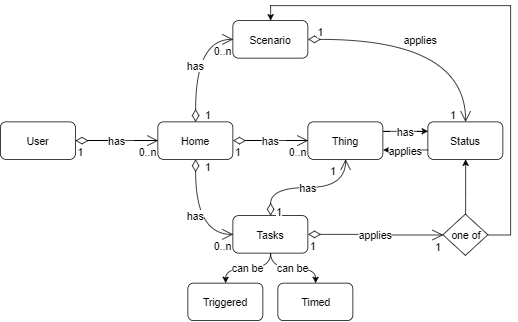
\includegraphics[scale=0.8]{img/domain.png}
  \caption{Modelo de Domínio}
\end{figure}

Resumidamente, o sistema possui vários utilizadores, sendo que cada um deles possui, portanto, uma ou mais casas e cada casa possui por sua vez um conjunto de dispositivos. Além disso, cada casa possui também os seus cenários e tarefas, podendo estas últimas serem ativadas com base em expressões temporais ou condicionantes baseadas noutros dispositivos do sistema. De seguida será apresentado um pequeno dicionário com o significado e função de cada entidade:

\paragraph*{User}
Representa o utilizador, que, como é normal, possui um email e uma password para autenticação. O utilizador é a entidade base do sistema, ou seja, qualquer outra entidade está diretamente ou indiretamente ligada a um utilizador.

Os dados do utilizador também serão utilizados como base para a autenticação e autorização. Ou seja, um utilizador não podem interagir com as entidades de outro utilizador.

\paragraph*{Home}
Representa a casa de um utilizador, contém dados para aceder à rede local e interage com os dispositivos lá instalados. Além disso, esta entidade também deverá possui uma referência ou um identificador do \textit{hub} instalado no espaço casa, algo que permite ao \textit{middleware} saber onde e como comunicar com os dispositivos desse espaço.

Todas as restantes entidades possuem uma associação direta ou indireta a um espaço casa.

\paragraph*{Thing}
Representa os dispositivos, contendo os dados necessários para efetuar comunicação com o mesmo. O \textit{hub} aceita uma lista de parâmetros para efetuar comunicação com um dispositivo compatível, mas como este é \textit{stateless}, não tem capacidade para os armazenar. Essa função pertence à \textit{api}, e é com recurso a esta entidade que se irá alcançar o objetivo pretendido.

Cada \textit{thing} possui dois parâmetros obrigatórios: tipo e subtipo. O tipo representa a funcionalidade geral do dispositivo, por exemplo, uma luz, uma fechadura ou um termóstato. O subtipo é referente à implementação do dispositivo, ou por outras palavras, o modelo do dispositivo. Neste caso a divisão entre tipos:

\begin{itemize}
    \item Things::Light - lâmpadas, dispositivos de iluminação
    \item Things::Lock - fechaduras, portas, portões
    \item Things::Thermostat - termostatos
    \item Things::Weather - estações meteorológicas, serviços de meteorologia
    \item Things::MotionSensor - sensores de movimento, alarmes
\end{itemize}

\newpage

Quanto aos subtipos, irão existir os seguintes:
\begin{itemize}
    \item Light - rest, coap, hue
    \item Lock - rest
    \item Thermostat - rest
    \item Weather - rest, owm
    \item MotionSensor - rest
\end{itemize}

Os subtipos \textit{rest} correspondem às simulações de dispositivos desenvolvidas no âmbito deste projeto. O \textit{coap} é também uma simulação, só que utiliza CoAP em vez de HTTP. O subtipo \textit{hue} corresponde às lâmpadas do \textit{Philips Hue} enquanto que o \textit{owm} corresponde ao serviço remoto de meteorologia \textit{OpenWeatherMap}.

\paragraph*{Status}
Representa o estado de um dispositivo. Os dispositivos retornam estas entidades mas estas também podem ser aplicadas ao dispositivo, efetivamente alterando o seu estado.

Isto permite-nos utilizar a arquitetura REST para alterar o estado dum dispositivo com base nos verbos HTTP, \textit{PUT} e \textit{GET}, onde o primeiro altera o estado e o segundo obtém o estado de um dispositivo.

\paragraph*{Scenario}
Representa um conjunto de estados que podem ser aplicados em conjunto. Tal como já foi referido anteriormente, podemos juntar estados que normalmente são aplicados ao mesmo tempo, como, desligar as luzes todas antes de o utilizador ir dormir, num só cenário que pode ser aplicado, simplificando muito a utilização da aplicação.

\paragraph*{Task}
Representam as tarefas, entidades que representam uma aplicação dum estado ou de um cenário com base numa condição (triggered ou timed). Isto permite definir as interações já referidas na introdução do problema, como, aplicar o cenário ''desligar luzes'' às 23:00, ou, ligar a luz da garagem quando o sensor de movimento lá colocado detetar movimento.

Como foi possível reparar nos exemplos referidos, temos dois tipos de tarefas, que serão agora apresentadas.

\paragraph*{Triggered}
Representam as tarefas condicionais, que são aplicadas com base no estado de um outro dispositivo presente neste sistema, como no exemplo acima referido, ligar a luz da garagem quando o sensor de movimento lá colocado detetar movimento.

\paragraph*{Timed}
Representam tarefas que são aplicadas com base numa dada expressão temporal. A tarefa ''aplicar o cenário desligar luzes às 23:00'' é deste tipo.

\section{Design}

De todos os componentes já referidos, apenas o \textit{hub} e a \textit{api} tiveram direito a um grande esforço no que toca ao desenho e elaboração da sua arquitetura utilizando diagramas, como dita o \textit{model driven development}. Os outros componentes como os simuladores de dispositivos são bastante simples e concisos, e não fazem parte do \textit{scope} da dissertação, são apenas ferramentas para demonstração. O mesmo se aplica à aplicação cliente e a componentes relacionados à demonstração, que apenas são um \textit{front-end} para demonstração do \textit{middleware}.


\subsection{Hub}

Como já foi visto anteriormente, o \textit{hub} tem como função agregar as APIs dos vários dispositivos de um espaço casa, numa API HTTP RESTful a ser consumida pelo \textit{core} do \textit{middleware}, a \textit{api}. No geral, foi concebida uma arquitetura seguindo o padrão MVC. Neste caso, o \textit{model} são os dispositivos, as \textit{views} os estado dos mesmos, enquanto que os \textit{controllers} aceitam os mais diversos parâmetros para estabelecer a comunicação com um dispositivo.

%
%
% THINGS
%
%

\paragraph*{Things}

Inicialmente foram definidas classes base para os diversos tipos de \textit{things} suportadas. Estas classes representam o estado de um dispositivo, indicando, por exemplo, se uma porta está fechada ou se uma luz está ligada. Serão suportadas os 5 tipos de \textit{things} já definidas no modelo de domínio: termóstato, sensor de movimento, fechadura, luz, estação de meteorologia. As \textit{things} são classes imutáveis, ou seja, o seu conteúdo não pode ser alterado dinamicamente, servindo apenas para representar um estado.

As \textit{things} não possuem muitas funcionalidades em comum, mas foram mesmo assim integradas num interface que possui dois métodos de utilidade. A partir de uma \textit{thing} deveremos obter a sua representação textual, por exemplo, a classe \textit{Lock} tem a representação textual \textit{lock}. Também deveremos obter a \textit{factory} que cria os serviços (definição dos mesmos mais à frente) que interagem com os dispositivos respetivos.

\begin{figure}[H]
  \centering
        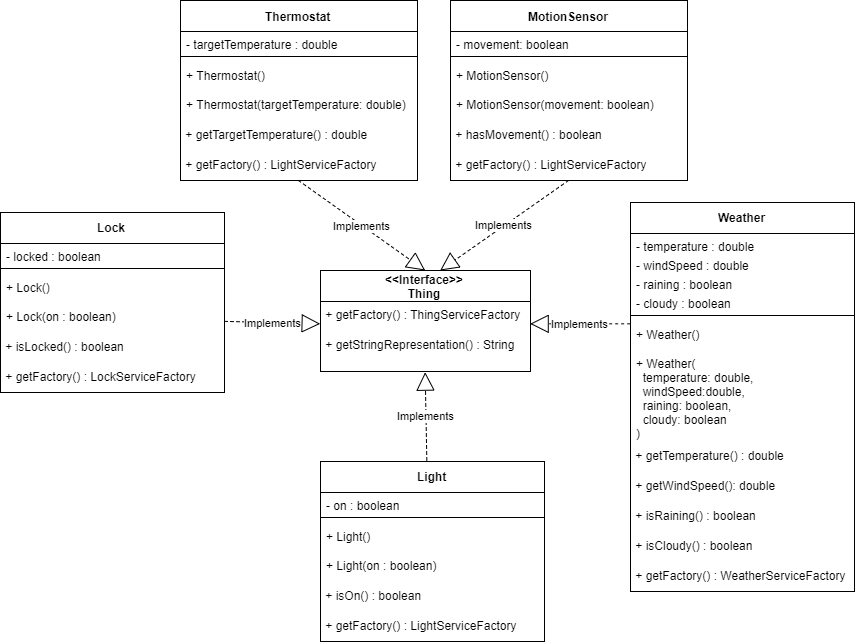
\includegraphics[scale=0.55]{img/hub-things.png}
  \caption{Diagrama de classes: \textit{Things}}
  \label{fig:things-hub}
\end{figure}

%
%
% SERVIÇOS
%
%

\paragraph*{Serviços}

Posto isto, teremos agora que idealizar a comunicação com os dispositivos. Neste caso faremos o uso de serviços, classes que possuem métodos para interagir com um dispositivo específico. Os serviços podem partilhar funcionalidade, como métodos para comunicação HTTP, e portanto esse tipo de funcionalidades estão encapsuladas em classes abstratas auxiliares. Neste caso, além do serviço base, temos também o serviço HTTP e CoAP, que possuem métodos auxiliares para comunicar com dispositivos que utilizem os protocolos respetivos.

Para cada subtipo de uma \textit{thing} deve existir um serviço. Como já vimos anteriormente, um subtipo representa um modelo especifico do dispositivo, e como cada subtipo exige um tipo de comunicação e interação diferente, é portanto necessário ter um serviço para cada um. No diagrama abaixo vemos os serviços para os subtipos da \textit{thing} do tipo \textit{light}, \textit{coap} e \textit{rest}.

\begin{figure}[H]
  \centering
        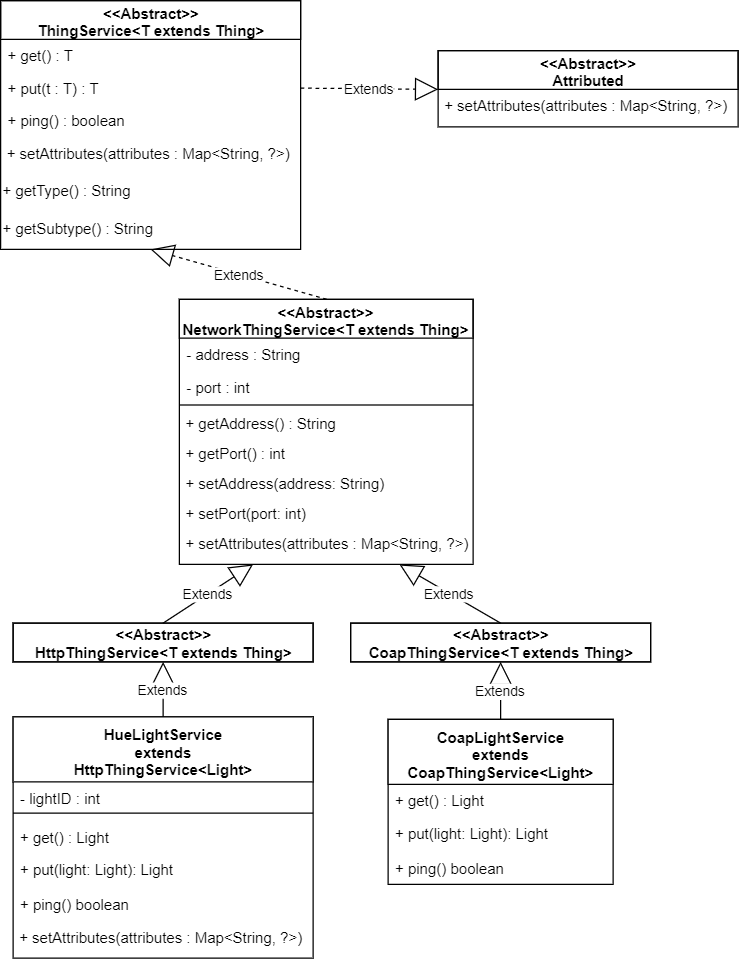
\includegraphics[scale=0.5]{img/hub-services.png}
  \caption{Diagrama de classes: Serviços}
\end{figure}

\newpage

Os restantes serviços serão de seguida enumerados, indicando as classes abstratas em que se baseiam:
\begin{itemize}
    \item \textit{rest light} -> RestLightService -> HttpThingService<Light>
    \item \textit{rest lock} -> RestLockService -> HttpThingService<Lock>
    \item \textit{rest thermostat} -> RestThermostatService -> HttpThingService<Thermostat>
    \item \textit{rest weather} -> RestWeatherService -> HttpThingService<Weather>
    \item \textit{owm weather} -> OWMWeatherService -> ThingService<Weather>
    \item \textit{rest motionsensor} -> RestMotionSensor -> HttpThingService<MotionSensor>
\end{itemize}

Os serviços possuem todos os parâmetros para efetuar comunicação com um dispositivo, nomeadamente o seu endereço, porta de acesso, entre outros. Estes parâmetros são fornecidos ao \textit{hub} nas chamadas à sua API e por ventura são passados aos serviços. O método \textit{setAttributes}, fornecido pela classe abstrata \textit{Attributed}, aceita um \textit{array} associativo, ou por outras palavras, um \textit{map}, que contém todos os atributos necessários para o seu funcionamento. Caso faltem atributos ou estes tenham formatos inválidos, deverá ser lançado um erro, uma exceção, ou um qualquer mecanismo da linguagem para assinalar \textit{inputs} inválidos. Apesar dos \textit{setters} e dos \textit{getters} presentes nos serviços, este método permite definir os atributos tendo apenas uma instância de \textit{ThingService}, sem saber a classe concreta da instância.

As instâncias concretas dos serviços não são de acesso público, apenas o interface base e as extensões abstratas. Decidiu-se proceder desta maneira para reduzir o acoplamento entre os serviços e as outras partes da aplicação, nomeadamente os \textit{controllers} que recebem parâmetros das chamadas à API e que comunicam com os dispositivos, utilizando os serviços para isso. Assim sendo, todos os serviços serão instanciados através de \textit{factories}, que recebem um subtipo e devolvem uma instância dum serviço referente ao subtipo dado. Mais uma vez, é por esta razão que definiu-se o método \textit{setAttributes}, para efetuar o \textit{assign} dos atributos sem ter acesso à classe específica de uma instância de um serviço.

A classe auxiliar \textit{Attributed}, em termos lógicos, basicamente assinala isto que já foi exposto, uma classe que permite mudar o seu estado interno, ou por outras palavras, os seus atributos, através de um \textit{map} entre o nome do atributo e o seu valor. Este comportamento foi extraído do serviço porque é utilizado noutros pontos da aplicação, nomeadamente a descoberta de serviços, que utiliza este mecanismo pelas mesmas razões supracitadas.

Os dispositivos do tipo base \textit{NetworkThingService} requerem todos um endereço e uma porta, que poderão ser passados à instância de um serviço através dos seus \textit{setters}, no entanto, não podemos fazer tal coisa, porque apenas interagimos com instâncias do tipo \textit{ThingService}, devido ao acesso privado das classes concretas. Para resolver isso utilizamos o método \textit{setAttributes}, como já se falou anteriormente. Classes que recorrem a parâmetros adicionais, como o \textit{HueLightService}, que faz uso do novo parâmetro \textit{lightID}, devem voltar a implementar o método \textit{setAttributes} para acomodar o novo parâmetro.

%
%
% FACTORIES
%
%

\paragraph*{\textit{Factories}}

Devido à abordagem à base de ''um serviço para um subtipo'', iremos ter várias classes concretas para cada um dos subtipos de dispositivos, portanto, irá ser utilizado o padrão \textit{abstract factory}, onde teremos várias fábricas de serviços, uma por cada tipo de dispositivo, para simplificar o processo de instanciação de serviços. Por exemplo, a fábrica do tipo ''luz'' é responsável por instanciar todos os serviços suportados por este tipo de dispositivo, aceitando um subtipo como parâmetro. As fábricas de objetos também devem ter um método de utilidade para ver se um dado subtipo é suportado. Além disso, o método \textit{create} deve, obviamente, finalizar com um erro quando o subtipo não é suportado.

\begin{figure}[H]
  \centering
        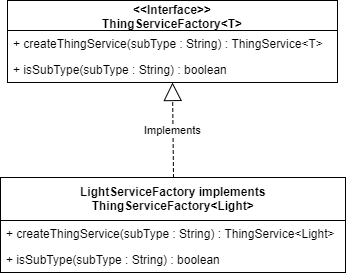
\includegraphics[scale=0.75]{img/hub-factories.png}
  \caption{Diagrama de classes: \textit{Factories}}
\end{figure}

Neste diagrama apenas está representada a \textit{LightServiceFactory}, mas todos os outros tipos de dispositivos tem fábricas com assinaturas semelhantes. O método \textit{create} retorna os serviços definidos acima, mas sem exportar os detalhes da classe concreta. Caso o método \textit{create} seja chamado com o subtipo \textit{hue} numa fábrica do tipo \textit{LightServiceFactory} a fábrica retorna um \textit{HueLightService} abstraído no interface \textit{ThingService<Light>}.

O interface base \textit{ThingServiceFactory} irá ter uma função vital nos \textit{controllers}, permitindo efetuar \textit{dependency injection} nestes, simplificando a operação dos mesmos. Assim, um \textit{controller} genérico consegue operar com qualquer tipo de dispositivo, baseado na \textit{factory} que o compõe.

%
%
% CONTROLLERS
%
%

\paragraph*{Controllers}

Seguindo a arquitetura MVC, já temos os componentes que representam o \textit{model}, neste caso as \textit{things} e os serviços, restando os \textit{controllers} e as \textit{views}. Os \textit{controllers} têm como função aceitar parâmetros provenientes da chamada à API, gerando alterações nos \textit{models}, ou mais concretamente, nos dispositivos. Além de gerar alterações, os \textit{controllers} também podem gerar as tais \textit{views}, representações dos estados dos dispositivos.

Tal como foi explicado no \textit{design} das \textit{factories}, os \textit{controllers} irão funcionar à base de \textit{dependency injection}, sendo compostos por uma \textit{ThingServiceFactory}, que irá ditar o tipo de dispositivos com que o \textit{controller} lida. Assim, tendo apenas uma definição base de um \textit{controller}, conseguimos trabalhar com todo o tipo de dispositivos, em vez de criar um \textit{controller} para cada tipo individual. Todo o objetivo de lidar com os genéricos, que consistem nestas classes parametrizadas com um tipo genérico \textit{T}, é atingir esta abstração, onde um \textit{controller} consegue lidar com vários tipos e subtipos de dispositivos, abstraindo todo este processo de seleção de serviços e passagem de parâmetros.

\begin{figure}[H]
  \centering
        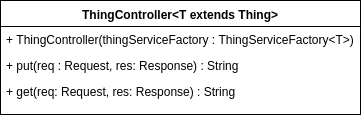
\includegraphics[scale=0.75]{img/hub-controllers.png}
  \caption{Diagrama de classes: \textit{Controllers}}
\end{figure}

O \textit{ThingController} é instanciado com uma \textit{ThingServiceFactory}, e possui dois métodos, \textit{get} e \textit{put}, que correspondem aos verbos HTTP GET e PUT, seguindo assim uma metodologia \textit{restful}, onde temos os recursos (\textit{things}) e utilizamos verbos HTTP para interagir com os recursos. O método \textit{put} tem como objetivo alterar o estado de um dispositivo dado um \textit{request} e uma \textit{response}, objetos que representam um pedido e uma resposta HTTP, normalmente de uma \textit{framework} de desenvolvimento de servidores web. O método \textit{get} serve apenas para retornar o estado atual de um dispositivo. Ambos estes métodos retornam uma \textit{string}, que representa a resposta da API em JSON a um qualquer pedido.

Internamente, o \textit{controller} recebe um pedido, retira o parâmetro subtipo dos parâmetros deste, cria um serviço através da \textit{factory}, utiliza o método \textit{setAttributes} atribuindo os restantes parâmetros, e depois chama o método correspondente no serviço, ou \textit{get} ou \textit{put}.

\newpage

%
%
% Descoberta de dispositivos
%
%

\paragraph*{Descoberta de Dispositivos}

Posto isto, temos os serviços que permitem estabelecer comunicação bidirecional com os dispositivos, faltando agora resolver o problema da descoberta de dispositivos na rede local. Uma parte muito importante de todo o paradigma da IoT e do espaço casa, uma vez que aumenta muito a facilidade de uso destes sistemas para o utilizador comum.

Inicialmente foram concebidas as classes para a descoberta de dispositivos, tendo como base o padrão \textit{strategy}, que define estratégias diferentes para resolver um dado problema. Isto traduz-se para uma classe abstrata base com um método \textit{perform}, que essencialmente leva a cabo a descoberta de dispositivos, utilizando uma fábrica de serviços e um subtipo como argumentos (passados através de um construtor).

As estratégias essencialmente dependem do subtipo de dispositivo utilizado. Dispositivos diferentes têm estratégias diferentes de descoberta, alguns podem utilizar UPNP, outros não, sendo necessário encontrar outras alternativas. Utilizando esta abordagem, é alcançável a elaboração de estratégias para cada um dos subtipos, mantendo esse processo transparente noutras camadas da aplicação, nomeadamente os \textit{controllers}.

\begin{figure}[H]
  \centering
        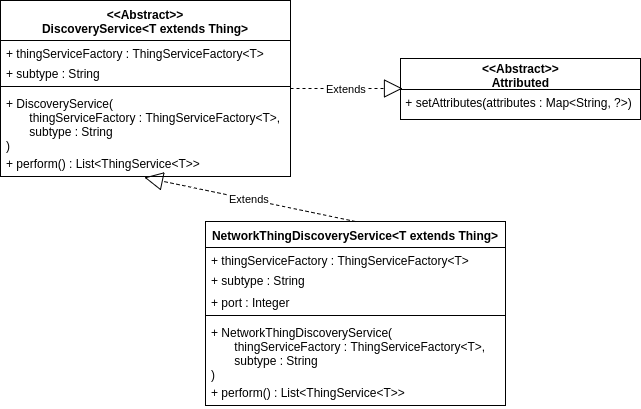
\includegraphics[scale=0.6]{img/hub-discovery.png}
  \caption{Diagrama de classes: \textit{Serviços de descoberta de dispositivos}}
\end{figure}

Neste caso apenas possuímos um único serviço de descoberta, \textit{NetworkThingDiscoveryService}, que descobre todo o tipo de dispositivos baseados no \textit{NetworkThingService}, ou seja, dispositivos que essencialmente atuam utilizando o protocolo IP, ou protocolos que se baseiam neste anterior, como HTTP ou CoAP, estando presentes na rede local do \textit{hub}. O \textit{NetworkThingDiscoveryService}, além do subtipo, que é necessário para todo o tipo de descobertas, também necessita de uma porta. Caso uma porta não seja passada como parâmetro será utilizada a porta ''default'' do protocolo utilizado (HTTP utiliza a porta 80 por exemplo).

Todos os subtipos são cobertos por esta estratégia de descoberta, exceto um, o subtipo \textit{owm}, que como se baseia num serviço remoto, não necessita de mecanismos de descoberta.

Concebida a arquitetura dos serviços, é preciso unir tudo e criar um \textit{controller} para expor esta funcionalidade, mas antes disso, ainda falta resolver de alguns detalhes. Primeiro, está novamente presente o problema encontrado nos \textit{thing services}, onde temos vários objetos distintos, tornando a sua instanciação um processo complexo. Para resolver isto, basta adicionar um outro método às \textit{factories}, que devolve uma implementação de um \textit{DiscoveryService} compatível com o \textit{subtipo}.

\begin{figure}[H]
  \centering
        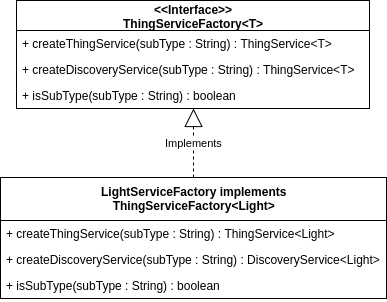
\includegraphics[scale=0.6]{img/hub-factories-discovery.png}
  \caption{Diagrama de classes: \textit{Factories atualizadas para suportar serviços de descoberta}}
\end{figure}

Assim, temos um mecanismo para obter a estratégia de descoberta de um determinado subtipo, simplificando todo esse processo da escolha da estratégia num novo método nas \textit{factories}. Os \textit{controllers} então só têm que trabalhar com instâncias de \textit{DiscoveryService}, utilizando o método \textit{setAttributes} da classe abstrata \textit{Attributed} para passar os parâmetros recebidos pelo \textit{controller}.

Por fim, efetua-se a conceção dos \textit{controllers} que expõem os serviços de descoberta. Estes \textit{controllers}, têm um funcionamento muito semelhante aos \textit{controllers} dos serviços das \textit{things}. Este tipo de \textit{controllers} só possui suporte para métodos do tipo GET, retornando uma lista de dispositivos disponíveis na rede local, e os parâmetros necessários para o seu funcionamento.

%depois mostramos como integramos isto num todo, mostrando o controller

O \textit{controller} extrai o subtipo fornecido nos parâmetros, utilizando a \textit{factory} para criar o \textit{discovery service} correspondente ao subtipo. Depois disto, são passados o restos dos parâmetros, como a porta de acesso no caso dos \textit{NetworkThingDiscoveryService}, utilizando o método \textit{setAttributes}. Por fim, após esta passagem de parâmetros é então executado o método \textit{perform} do serviço de descoberta, retornando a lista de dispositivos encontrados na rede do \textit{hub}.

%
%
% VISAO GERAL
%
%

\paragraph*{\textit{API HTTP} - Visão Geral}

Concluindo o desenho arquitetural, agora prossegue-se à definição da API HTTP que irá ser consumida pelo \textit{core} do \textit{middleware}.

Uma API HTTP é normalmente constituída por recursos, identificados por um URL, e pelas ações disponíveis em cada um. Uma ação é identificada pelo verbo HTTP, como já foi demonstrado no \textit{design} dos \textit{controllers}. Exemplos de verbos HTTP podem ser o GET, que tem como função a simples obtenção de um recurso, e o PUT, que tem como função a alteração de um recurso existente.

Posto isto, temos primeiros os URLs de acesso aos dispositivos, cada um com suporte para operações GET e PUT, onde o GET retorna o estado do dispositivo e o PUT permite alterar o estado do dispositivo.

\begin{verbatim}
            /devices/lights
            /devices/locks
            /devices/thermostats
            /devices/weather
            /devices/motionsensors
\end{verbatim}

Os parâmetros de acesso, como o endereço IP do dispositivo, devem ser passados à API através de uma \textit{query string}, adicionada ao URL. Estes parâmetros são recolhidos pelo \textit{controller} e posteriormente passados para os serviços respetivos, quer os serviços das \textit{things} ou de descoberta.

\begin{verbatim}
            /devices/light?subtype=rest&address=foo.light.local&port=80
\end{verbatim}

Este exemplo permite estabelecer contacto com um dispositivo do tipo \textit{light} e do subtipo \textit{rest}, utilizando o endereço \textit{foo.light.local} e a porta 80 como parâmetros de rede. Internamente, este pedido e os seus parâmetros são passados ao \textit{ThingController} e depois este trata de completar a operação em causa.

Com ambos os verbos HTTP, a resposta a uma chamada da API do \textit{hub} é um objeto do tipo \textit{thing} serializado para JSON. O corpo dos pedidos do tipo PUT também deve seguir a mesma estrutura e formato. De seguida podemos observar um objeto do tipo \textit{light} no formato JSON.

\begin{verbatim}
            {
                "on" : false
            }
\end{verbatim}

Todas as variáveis de instância de qualquer \textit{thing} são convertidas na serialização, de modo a que as restantes representações em JSON dos outros tipos podem ser inferidas através da figura \ref{fig:things-hub}.

As rotas para interagir com os serviços de descoberta têm o seguinte formato:

\begin{verbatim}
            /devices/lights/discover
            /devices/locks/discover
            /devices/thermostats/discover
            /devices/weather/discover
            /devices/motionsensors/discover
\end{verbatim}

Para encontrar um dispositivo basta efetuar um pedido GET para uma destas rotas, fornecendo como parâmetros um subtipo mais outro subconjunto de parâmetros dependendo do subtipo em questão.

\begin{verbatim}
            /devices/light/discover?subtype=rest&port=80
\end{verbatim}

Este pedido procura por dispositivos do tipo \textit{rest} que estejam a operar na porta 80. Um exemplo de resposta tem o seguinte formato:

\begin{verbatim}
            [
                {
                    "address":"foo.light.local",
                    "port":80,
                    "subtype":"rest",
                    "type":"Things::Light"
                }
            ]
\end{verbatim}

Basicamente trata-se de uma lista JSON com os dispositivos encontrados. Internamente são os serviços que são serializados para JSON, serializando os atributos relevantes ao funcionamento do serviço, neste caso \textit{address}, \textit{port}, \textit{subtype} e \textit{type}.
\subsection{Api}

A \textit{api} é a parte central do projeto, contendo toda a lógica e funcionalidades para responder aos problemas encontrados. Como já foi explicado anteriormente, a \textit{api} irá adotar uma arquitetura \textit{REST}, utilizando HTTP como protocolo de transporte. Nesta secção será delineada a arquitetura interna da \textit{api} e depois os vários \textit{endpoints} e métodos da aplicação.

Como arquitetura deverá ser adotado o modelo MVC, que efetua a correta separação entre as três camadas essenciais de uma aplicação \textit{enterprise}, dados, lógica de negócio e apresentação, que mapeia para os conceitos, \textit{model}, \textit{controller}, \textit{view}. Este padrão é bastante predominante em aplicações web, inclusive APIs REST, porque torna muito mais manutenível e legível, um sistema complexo com vários tipos de modelos e operações. Além desta abordagem será utilizada uma \textit{service layer}, para efetuar operações complicadas de mais para aparecer num \textit{controller}.

Neste cenário, os \textit{models} são apenas \textit{placeholders} para os dados vindos da base de dados, sendo utilizado qualquer tipo de camada ORM para efetuar o mapeamento de dados. Os \textit{controllers} têm como objetivo receber os parâmetros dos pedidos à API, efetuando operações necessárias na base de dados, através da camada ORM, recorrendo a \textit{service objects} quando a lógica se torna complexa demais.

Ao contrário do \textit{hub}, que utilizava apenas um subconjunto muito simples da arquitetura REST, esta parte do projeto já aumenta bastante de complexidade, e portanto serão detalhadas as ações REST utilizadas.
Como é normal em \textit{designs} REST, as aplicações são divididas em recursos, como por exemplo ''utilizadores'' ou ''casas'', e cada recurso possui métodos CRUD para serem manipulados. Utilizando HTTP, os recursos são representados por URLs e são utilizados os métodos do protocolo para manipular os recursos. De seguida, uma especificação das ações REST mais comuns a sua implementação em HTTP.

\begin{table}[H]
\centering
  \begin{tabularx}{\textwidth}{ | l | c | c | X | }
    \hline
    Ação & Método HTTP & Identificador de Recurso & Descrição\\  \hline
    INDEX & GET & /recurso & Obtém todos os elementos presentes neste recurso\\ \hline
    SHOW & GET & /recurso/:id & Obtém um elemento identificado pelo parâmetro variável ''id'' \\ \hline
    CREATE & POST & /recurso & Adiciona um novo elemento ao recurso com os parâmetros fornecidos no \textit{body} do pedido HTTP\\ \hline
    UPDATE & PUT/PATCH & /recurso/:id & Atualiza um elemento identificado pelo parâmetro variável ''id'' com os parâmetros fornecidos no \textit{body} do pedido HTTP \\ \hline
    DESTROY & DELETE & /recurso/:id & Apaga um elemento identificado pelo parâmetro variável ''id'' \\ \hline
  \end{tabularx}
  \caption{Ações REST}
\end{table}

Portanto, esta aplicação é composta por recursos, cada recurso sendo manipulado por um \textit{controller}, fazendo alterações no respetivo \textit{model}, sendo as suas alterações representadas pela sua \textit{view}, que neste caso são simples classes de utilidade que serializam objetos para JSON. Os \textit{controllers} serão compostos pelas ações da tabela acima, sendo cada ação um método no \textit{controller}, depois cada método será mapeado para uma rota, que é uma combinação de um URL com um método HTTP, semelhante ao que vimos na tabela 2.


% FAZER UM DIAGRAMA AQUI SFF



\subsubsection{Recursos}

Os recursos que compõem esta parte do projeto são baseados no modelo de domínio feito anteriormente, havendo quase um mapeamento perfeito do modelo para recursos da aplicação. De seguida, serão apresentados os diferentes recursos, as rotas de acesso aos mesmos, assim como o formato dos elementos dos diferentes recursos. O formato dos elementos segue os mesmos formatos da especificação JSON, porque de facto são objetos em JSON, tendo os seguintes tipos:
\begin{itemize}
    \item string
    \item number
    \item object (outro objeto JSON)
    \item array
    \item boolean
    \item null
\end{itemize}

\paragraph*{Users}

Segue exatamente a mesma lógica da entidade \textit{User} do modelo de domínio, representado os utilizadores da aplicação e servindo como base para os mecanismos de autenticação.

Este recurso é um pouco diferente do habitual, sendo um recurso singular, ou seja, não tem nenhum identificador nem mecanismos de listagem (ação \textit{index}). O objetivo é que este recurso seja utilizado para o registo de novos utilizadores assim como a obtenção e atualização dos mesmos. O identificador deverá ser o próprio mecanismo de autenticação, através de um \textit{token} presente nos cabeçalhos dos pedidos.

\textbf{Ações}
\begin{itemize}
    \item POST /users -> CREATE
    \item GET /users/me -> SHOW
    \item PUT/PATCH /users/me -> UPDATE
\end{itemize}

\textbf{Formato dos objetos de entrada}
\begin{itemize}
    \item name - string
    \item email - string
    \item password - string
    \item password{\_}confirmation - string
\end{itemize}

\textbf{Formato dos objetos de saída}
\begin{itemize}
    \item id - number
    \item name - string
    \item email - string
\end{itemize}

\paragraph*{Homes}

Este recurso representam as diversas casas dos utilizadores, contendo informação para interagir com os dispositivos dentro da casa do utilizador através dum \textit{hub}. Essencialmente, uma casa é o objeto representativo do \textit{hub}, sendo o interface de comunicação entre o utilizador e os seus dispositivos. De notar a existência de um \textit{id} no objeto de saída, que é dado ao objeto depois da sua gravação na base de dados.

\textbf{Ações}
\begin{itemize}
    \item GET /homes -> INDEX
    \item POST /homes -> CREATE
    \item GET /homes/:id -> SHOW
    \item PUT/PATCH /homes/:id -> UPDATE
    \item DELETE /homes/:id -> DESTROY
\end{itemize}

\textbf{Formato dos objetos de entrada}
\begin{itemize}
    \item name - string
    \item location - string
    \item tunnel - object
\end{itemize}

\textbf{Formato dos objetos de saída}
\begin{itemize}
    \item id - number
    \item name - string
    \item location - string
    \item tunnel - object
    \item ip{\_}address - string
\end{itemize}

Os atributos \textit{name} e \textit{location} são apenas utilidades para o próprio utilizador categorizar a sua casa na aplicação, já o \textit{tunnel} é um objeto que contém informação para conectar com o \textit{hub} na casa do utilizador. Internamente, a \textit{api} atribui um endereço IP á casa, o mesmo IP proveniente do pedido HTTP. Na próxima secção, onde irão ser detalhados os aspetos da implementação mais importantes, irá ser delineado a tecnologia utilizada na tunelização entre o \textit{hub} e a \textit{api}.

\paragraph*{Things}

Também conhecido como ''coisas'', é um termo utilizado para definir os dispositivos dos utilizadores, presentes numa das suas casas. Cada \textit{thing} possui as mesmas informações que são enviadas para os \textit{ThingServices} no \textit{hub}, ou seja, parâmetros como o \textit{subtype}, \textit{address} entre outros são todos armazenados neste recurso. Os dispositivos pertencem a uma casa e portanto a um utilizador (via esta ultima relação).

\textbf{Ações}
\begin{itemize}
    \item GET /homes/:home{\_}id/things -> INDEX
    \item POST /homes/:homes{\_}id/things -> CREATE
    \item GET /things/:id -> SHOW
    \item PUT/PATCH /things/:id -> UPDATE
    \item DELETE /things/:id -> DESTROY
\end{itemize}

Nestas ações já se pode ver \textit{nesting} de rotas, uma vez que é necessário saber a que casa pertencem os dispositivos. Este \textit{nesting} é superficial, ou seja, se fornecido o \textit{id} de um dispositivo já não é preciso fornecer o \textit{id} de uma casa.

\textbf{Formato dos objetos de entrada}
\begin{itemize}
    \item name - string
    \item type - string
    \item subtype - string
    \item connection{\_}info - object
\end{itemize}

\textbf{Formato dos objetos de saída}
\begin{itemize}
    \item id - number
    \item name - string
    \item type - string
    \item subtype - string
    \item connection{\_}info - object
\end{itemize}

O atributo \textit{name}, mais uma vez, só serve para caracterizar o dispositivo, não tendo nenhuma funcionalidade em específico. O tipo e subtipo são essenciais para comunicar com os dispositivos através do \textit{hub}, sendo os restantes parâmetros que variam de acordo com o subtipo fornecidos através do atributo variável \textit{connection{\_}info}.

As \textit{things} terão métodos para obter e alterar o seu estado, \textit{getStatus} e \textit{putStatus} utilizando o objeto \textit{tunnel} de uma \textit{home} para estabelecer conexão. Estes métodos serão utilizados noutro recurso para expor estes mecanismos na \textit{api}.

\paragraph*{Things Status}

Este recurso permite obter os estados dos dispositivos, evocando os métodos do \textit{get} e \textit{put} dos \textit{ThingServices} presentes no \textit{hub}. Internamente é efetuada uma chamada à API do \textit{hub} através do túnel presente na \textit{home} da \textit{thing} desejada.

\textbf{Ações}
\begin{itemize}
    \item GET /things/:thing{\_}id/status -> INDEX
    \item PUT/PATCH /things/:thing{\_}id/status -> UPDATE
\end{itemize}

O formato dos objetos depende do tipo da \textit{thing} fornecida, estes formatos podem ser inferidos através da figura \ref{fig:things-hub}, que apresenta os tipos diferentes de \textit{things} e os seus atributos.

\paragraph*{Things Discovery}

De uma maneira semelhante ao recurso anterior, este permite aceder ao serviço de descoberta de dispositivos presente num \textit{hub}, invocando a API deste a partir do \textit{tunnel}.

\textbf{Ações}
\begin{itemize}
    \item GET /homes/:home{\_}id/discovery -> INDEX
\end{itemize}

O formato das respostas é exatamente igual às respostas do \textit{hub}, que podem ser vistas na ultima secção.

%SENARIOS

\paragraph*{Scenarios}

Os cenários, como já vimos anteriormente, são um conjunto de dispositivos e os respetivos estados que devem ser lhes aplicado. Essencialmente este recurso é o ponto de partida para a funcionalidade dos cenários, que ainda é composta por mais outros dois recursos. Cada cenário pertence a uma casa.

\textbf{Ações}
\begin{itemize}
    \item GET /homes/:home{\_}id/scenarios -> INDEX
    \item POST /homes/:homes{\_}id/scenarios -> CREATE
    \item GET /scenarios/:id -> SHOW
    \item PUT/PATCH /scenarios/:id -> UPDATE
    \item DELETE /scenarios/:id -> DESTROY
\end{itemize}

\textbf{Formato dos objetos de entrada}
\begin{itemize}
    \item name - string
\end{itemize}

\textbf{Formato dos objetos de saída}
\begin{itemize}
    \item id - number
    \item name - string
    \item scenario{\_}things - array
\end{itemize}

O atributo \textit{name}, tal como nos recursos anteriores, é apenas um campo identificativo útil para o utilizador nomear os seus cenários. De notar que no objeto de saída existe um atributo do tipo \textit{array} chamado de \textit{scenario{\_}things}, que na verdade consiste noutro recurso que vamos ver já de seguida.

\paragraph*{Scenario Things}

Nos cenários é referido que os mesmos consistem num conjunto de dispositivos e os respetivos estados, no entanto estes não foram mencionados, isto porque foi necessário colocar-los noutro recurso devido à sua pluralidade. Um \textit{scenario thing} consiste então na combinação de um estado com um dispositivo, sendo o estado um elemento variável de formato igual aos objetos do recurso \textit{Thing Status}. Em linguagem natural, uma instância de \textit{scenario thing} pode ser ''uma luz apagada'' ou ''uma porta aberta''. Tendo este recurso separado dos cenários podemos então combinar várias \textit{scenario things} num só \textit{scenario} podendo ao mesmo tempo ''fechar uma porta'' e ''ligar uma luz''. Um \textit{scenario thing} pertence então a um \textit{scenario}, podendo este último ter vários \textit{scenario things}.

\textbf{Ações}
\begin{itemize}
    \item GET /scenarios/:scenarios{\_}id/things -> INDEX
    \item POST /scenarios/:scenarios{\_}id/things -> CREATE
    \item GET /scenarios/:scenarios{\_}id/things/:id -> SHOW
    \item PUT/PATCH /scenarios/:scenarios{\_}id/things/:id -> UPDATE
    \item DELETE /scenarios/:scenarios{\_}id/things/:id -> DESTROY
\end{itemize}

\textbf{Formato dos objetos de entrada}
\begin{itemize}
    \item status - object
    \item thing{\_}id - number
\end{itemize}

\textbf{Formato dos objetos de saída}
\begin{itemize}
    \item id - number
    \item status - object
    \item thing - object
\end{itemize}

\paragraph*{Scenario Applier}

No que toca a cenários só falta mesmo um mecanismo para aplicar o mesmo. Este exemplo também demonstra bem a diferença entre REST e outras abordagens como SOAP. Em SOAP provavelmente teríamos um método remoto \textit{applyScenario} que seria invocado pelo cliente, no entanto, em REST apenas temos recursos e métodos os métodos base do HTTP, e portanto criámos um recurso chamado de \textit{Scenario Applier}, chamando o método POST no mesmo (porque se está a invocar alterações no servidor, portanto é boa prática usar POST). Este é um dos poucos recursos sem modelos ou persistência de dados associados.

\textbf{Ações}
\begin{itemize}
    \item POST /scenarios/:scenarios{\_}id/apply -> CREATE
\end{itemize}

Este recurso não tem nenhum tipo de objeto de entrada ou saída, enviando o \textit{body} dos pedidos em branco, respondendo apenas com os \textit{status codes} apropriados.

\paragraph*{Timed Tasks}

Durante a fase conceptual já foi definido o conceito de tarefas, ou \textit{tasks}, basicamente consiste na aplicação de um estado a um dispositivo, ou de vários estados a vários dispositivos (um cenário no fundo), de acordo com uma dada condição. Neste caso a condição é uma expressão temporal, que indica quando uma dada tarefa deve ser aplicada.

Para definir a expressão temporal irão ser utilizadas expressões \textit{cron}, que permitem grande flexibilidade na temporização de tarefas. Desta maneira conseguimos definir temporizadores bastante flexíveis e precisos como pode ser notado nos seguintes exemplos:
\begin{itemize}
    \item 0 9 * * * - todos os dias às 9 horas
    \item 0 10 * * 1 - todas as segundas às 10h
    \item 0 20 * * 1,5 - todas as segundas e sextas às 20h
    \item */5 * * * * - de 5 em 5 minutos
\end{itemize}

As expressões \textit{cron} indicam portanto intervalos de tempo podendo escolher os dias da semana e do mês onde as mesmas correm assim como os minutos e horas a que as mesmas devem correr. Recorrendo ao comando \textit{man} \footnote{\url{https://linux.die.net/man/1/crontab}} de sistemas UNIX podemos saber mais sobre o \textit{crontab}, o \textit{scheduler} de tarefas destes sistemas, que usam estas tais expressões para definir os intervalos a que as tarefas devem ser executadas.

\textbf{Ações}
\begin{itemize}
    \item GET /homes/:home{\_}id/tasks/timed -> INDEX
    \item POST /homes/:homes{\_}id/tasks/timed -> CREATE
    \item GET /tasks/timed/:id -> SHOW
    \item PUT/PATCH /tasks/timed/:id -> UPDATE
    \item DELETE /tasks/timed/:id -> DESTROY
\end{itemize}

\textbf{Formato dos objetos de entrada}
\begin{itemize}
    \item id - number
    \item cron - string
    \item thing{\_}id - number 
    \item status{\_}to{\_}apply - object
    \item scenario{\_}id - number
\end{itemize}

\textbf{Formato dos objetos de saída}
\begin{itemize}
    \item id - number
    \item cron - string
    \item next{\_}run - string
    \item thing - object
    \item status{\_}to{\_}apply - object
    \item scenario - object
\end{itemize}

Os objetos pertencentes a este recurso podem ativar um cenário ou uma única \textit{thing}, e não ambos ao mesmo tempo, portanto não se pode fornecer um \textit{scenario{\_}id} ao mesmo tempo que se fornece um \textit{thing{\_}id}. Assim temos dois tipos de objetos de entrada, uns com o ID do cenário a aplicar, e outros com um ID de um dispositivo mais o respetivo estado a aplicar, \textit{status{\_}to{\_}apply}. O atributo \textit{cron} é uma expressão temporal como já vimos em cima que define quando a tarefa vai ser aplicada.

Nos objetos de saída temos ainda mais um atributo bastante útil, chamado de \textit{next{\_}run}, que contém a data da próxima execução desta tarefa.

\paragraph*{Triggered Tasks}

Já possuímos tarefas encadeadas à base de tempo, faltando o outro tipo que são ativadas com base no valor de um certo dispositivo. Nestes cenários de IoT aplicados no espaço casa, é muito comum os utilizadores quererem que certos comportamentos sejam programados de acordo com certas mudanças no ambiente, por exemplo, um cenário comum é ligar luzes utilizando sensores de movimento, o que é possível fazer no nosso caso porque possuímos o tipo base para cada um deste dispositivos.

Portanto para alcançar esta funcionalidade foi criado este recurso, que permite aplicar uma dada tarefa com base no valor do estado de um outro dispositivo. Para isso, o utilizador tem que escolher um dispositivo a monitorizar e o estado que desencadeie a execução da tarefa. Internamente a aplicação vai fazendo uma comparação lógica com o estado do dispositivo fornecido com o estado atual do mesmo, e quando essa comparação tiver um valor verdadeiro a tarefa é aplicada.

Tal como as tarefas temporizadas, este novo tipo também segue as mesmas regras quanto a escolha de um cenário ou um dispositivo como alvo de ativação.

\textbf{Ações}
\begin{itemize}
    \item GET /homes/:home{\_}id/tasks/triggered -> INDEX
    \item POST /homes/:homes{\_}id/tasks/triggered -> CREATE
    \item GET /tasks/triggered/:id -> SHOW
    \item PUT/PATCH /tasks/triggered/:id -> UPDATE
    \item DELETE /tasks/triggered/:id -> DESTROY
\end{itemize}

\textbf{Formato dos objetos de entrada}
\begin{itemize}
    \item id - number
    \item thing{\_}to{\_}compare{\_}id - number
    \item status{\_}to{\_}compare - object
    \item comparator - string
    \item thing{\_}id - number 
    \item status{\_}to{\_}apply - object
    \item scenario{\_}id - number
\end{itemize}

\textbf{Formato dos objetos de saída}
\begin{itemize}
    \item id - number
    \item thing{\_}to{\_}compare - object
    \item status{\_}to{\_}compare - object
    \item comparator - string
    \item next{\_}run - string
    \item thing - object
    \item status{\_}to{\_}apply - object
    \item scenario - object
\end{itemize}

Os objetos deste recurso possuem todos um \textit{thing{\_}to{\_}compare{\_}id}, que indica o dispositivo que queremos monitorizar, um \textit{status{\_}to{\_}compare{\_}id}, que indica o estado que queremos utilizar na comparação com o dispositivo monitorizado, e por fim, um \textit{comparator}, um operador lógico que deve ser utilizado na comparação entre o dispositivo monitorizado e o seu estado atual com o \textit{status{\_}to{\_}compare} fornecido neste objeto.

Além destes atributos, este tipo de tarefas também contêm os alvos de ativação como as tarefas temporizadas, ou seja, ou um cenário ou um dispositivo com um estado a aplicar.

